\documentclass[12pt]{book}
\usepackage{parskip}
\usepackage{titlesec}
\usepackage{graphicx}
\usepackage{cleveref}
\usepackage{amsmath}
\usepackage[a4paper, inner=2cm, outer=3cm, top=4cm, bottom=3cm, bindingoffset=2cm]{geometry}
\usepackage[doublespacing]{setspace}
\usepackage{booktabs}
\usepackage{subcaption}
\usepackage{fixltx2e} 
\usepackage{fancyhdr}
\usepackage{setspace}
\usepackage[colorlinks=true,linkcolor=black]{hyperref}
\usepackage[T1,OT1]{fontenc}
\renewcommand{\chaptername}{Bab}
\renewcommand{\contentsname}{Daftar Isi}
\renewcommand{\figurename}{Gambar}
\renewcommand{\listfigurename}{Daftar Gambar}

\usepackage{titlesec, blindtext, color}
\definecolor{gray75}{gray}{0.6}
\newcommand{\hsp}{\hspace{5pt}}
%\titleformat{\chapter}[hang]{\Huge\bfseries}{\thechapter\hsp\textcolor{gray75}{|}\hsp}{0pt}{\Huge\bfseries}
%Options: Sonny, Lenny, Glenn, Conny, Rejne, Bjarne, Bjornstrup
\usepackage[Lenny]{fncychap}
\pagestyle{fancy}
\fancyhf{}
\fancyhead[LE]{\leftmark}
\fancyhead[RO]{\nouppercase{\rightmark}}
\fancyfoot[LE,RO]{\thepage}
%===============================================================
\begin{document}
\begin{titlepage}
Modul Ajar\\
\textsc{\Huge Sistem Linier 2}\\[13cm]
Penyusun:\\
Dwi Prananto, ST, MSc\\
{\large
Universitas Panca Marga Probolinggo} \\
Bagus Tris Atmaja, ST, MT \\
{\large
Institut Teknologi Sepuluh Nopember\\}
\end{titlepage}
\tableofcontents{}\listoffigures
%==============================================================
\chapter{Sinyal dan Sistem}

\section{Pengantar}
Sinyal dan sistem merupakan sebuah kesatuan yang saling berhubungan satu sama lain. Sinyal merupakan pola-pola bervariasi yang berubah terhadap satu atau lebih variabel bebas, yang berisi informasi tentang perilaku atau sifat dari suatu fenomena tertentu. Sistem akan menerima sinyal untuk kemudian mengelola, mengolahnya sehingga menhasilkan keluaran atau tanggapan berupa sinyal lain ataupun perilaku atau sifat tertentu sesuai keinginan. Penerapan sinyal dan sistem ada dalam banyak bidang yang bervariasi mulai dari teknologi komunikasi, elektronika, komputer, pembangkit energi, pengolahan suara untuk musik, transportasi, sampai kendali otomatis pada proses-proses di industri. Masih banyak lagi penerapan sinyal dan sistem dalam kehidupan sehari-hari yang kita sadari atau tidak telah kita gunakan secara rutin dalam kehidupan kita. Penerapan-penerapan tersebut kesemuanya memiliki pola dan ciri mendasar seperti yang telah dijabarkan pada awal paragraf. Contoh sederhananya adalah mobil. Mobil bergerak dan melaju dengan kecepatan tertentu akibat adanya injakan dari pedal gas, dalam hal ini injakan pada pedal gas merupakan sinyal masukan bagi sistem mobil dan sistem mobil melalui proses mekanis dan termodinamik pada mesinnya akan menhasilkan tanggapan berupa laju mobil yang sesuai dengan seberapa dalam injakan pedal gas. Contoh lain terdapat pada rangkaian listrik, dimana sinyal masukan berupa arus dan tegangan listrik yang berubah terhadap waktu pada sistem rangkaian listrik yang dapat berupa komponen-komponen elektronik dan elektrik seperi resistor, kapasitor dan lain-lain akan menghasilkan tanggapan berupa arus dan tegangan yang berbeda sesuai dengan yang diinginkan. 

\begin{figure}[!h]
\centering
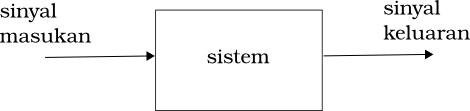
\includegraphics[scale=0.7]{pict/sinyalsistem}
\caption{Representasi konsep sinyal dan sistem dalam diagram blok}\label{sinyalsistem}
\end{figure}

Konsep sinyal dan sistem muncul dalam dalam berbagai aplikasi yang berbeda bergantung pada bagaimana pengunaan konsep tersebut. Konsep sinyal dan sistem dapat digunakan untuk mengkaraterisasi sebuah sistem. Mengkarakterisasi berarti membaca karakter atau sifat dari sebuah sistem tertentu dengan cara memberikan sinyal masukan yang bervariasi dan membaca bagaimana sistem menanggapai masukan yang bervariasi tersebut. Hal ini seperti apabila kita mempunyai sebuah kotak hitam yang kita tidak tahu sepeti apa sifat dan bagaimana kotak hitam tersebut bekerja. Dengan memberikan masukan bervariasi terhadap kotak hitam tersebut maka akan dapat diperoleh keluaran barupa tanggapan yang berbeda dengan masukan, sehingga dengan ini kita dapat mengetahui apa dan bagaimana kotak hitam misterius ini berperilaku atau bekerja. Konsep sinyal dan sistem juga dapat digunakan untuk melakukan pemrosesan terhadap sinyal tertentu agar diperoleh keluaran sinyal sesuai yang diharapkan atau untuk menghilangkan sinyal yang tidak diinginkan. Contohnya adalah dalam sistem \textit{noise canceling} (NC) atau pembatal bising. Dalam sistem NC yang biasa digunakan pada speaker, bising atau suara mengganggu yang tidak diinginkan dari dapat diredam sedemikian hinga sehingga suara atau bunyi yang keluar dari \textit{speaker} adalah ahanya suara yang diharapkan. Sistem NC akan membangkitkan suara dengan frekuensi tertentu yang sama dengan suara bising tertentu tetapai dengan fase yang berbeda sehingga melalui proses interferensi suara bising dapat diredam. 

\begin{figure}[!h]
\centering
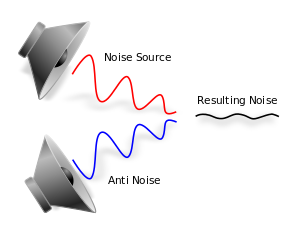
\includegraphics[scale=0.7]{pict/300px-Active_Noise_Reduction}
\caption{Grafik bagaimana sistem NC dapat meredam bising.  [Kredit gambar: wikimedia commons]}\label{NC}
\end{figure}
     
Penggunaan lain dari konsep sinyal dan sistem adalah pada proses kendali otomatis (\textit{automatic control system}). Sistem seperti ini digunakan untuk mengendalikan besaran-besaran fisis tertentu seperti suhu, kelembaban, ketinggian air, kecepatan aliran, arah gerak benda dan lain-lain agar besaran fisis ini berada pada nilai tertentu sesuai dengan yang diharapkan. Sistem ini umumnya tersusun atas gabungan dari beberapa sistem. Dalam sistem kendali otomatis sinyal yang diberikan oleh sensor, yang bertugas untuk merasakan suatu besaran fisis, akan digunakan oleh sistem untuk melakukan pengaturan terhadap besaran fisis seperti suhu, kecepatan laju aliran, pergerakan motor, dan lain-lain. Di dalam sistem ini sensor juga berperan sebagai pemberi umpan balik bagi sistem sehingga sistem dapat menjaga besaran fisis yang dikendalikan pada tingkat atau kuantitas yang diharapkan. Contoh dari sistem kendali otomatis ini adalah antara lain sistem \textit{autopilot} yang ada di pesawat untuk mengendalikan pesawat agar terbang pada jalur arah dan ketinggian tertentu. Contoh lain adalah sistem kendali suhu ruangan yang ada pada alat pengkondisi ruang (\textit{air conditioning}/AC), AC akan mengatur hembusan dan temperatur udara yang akan keluar dari AC sebagai tanggapan dari pembacaan sensor terhadap suhu ruangan.  

\begin{figure}[!h]
\centering

\includegraphics[scale=0.13]{pict/2000px-Feedback_Loop}
\caption{Diagram blok sistem dengan umpan balik sederhana. $X$ merupakan sinyal masukan, $Y$ merupakan sinyal tanggapan, $P_2$ adalah komponen yang memberikan umpan balik ke sistem. [Kredit gambar: wikimedia commons]}\label{umpanbalik}
\end{figure}

Untuk dapat melakukan analisis terhadap sinyal dan sistem, dibutuhkan seperangkat kerangka kerja analitis yang menggambarkan dan merepresentasikan secara matematis sinyal dan sistem tertentu yang dapat digunakan untuk memecahkan berbagai macam masalah. 
       
\section{Sinyal Waktu-Kontinu dan Sinyal Waktu-Diskrit}
Informasi dalam sebuah sinyal direpresentasikan oleh pola-pola bervariasi yang berubah terhadap variabel bebas tertentu seperti waktu. Pola-pola bervariasi yang didapatkan dari perekaman suara melalui mikrofon merupakan salah satu contoh representasi sinyal. Variasi tekanan akustik yang dirasakan oleh sensor yang ada pada mikrofon, yang sekaligus merubahnya menjadi sinyal-sinyal listrik, sebagai fungsi waktu direpresentasikan ke dalam pola-pola bervariasi tertentu. Pola-pola yang berbeda berisi informasi tentang suara-suara/kata-kata yang berbeda pula.  

\begin{figure}[!h]
\centering
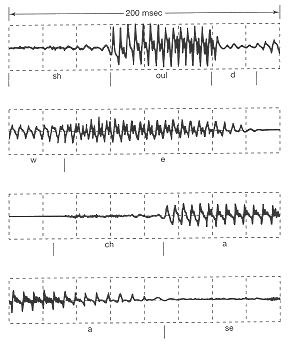
\includegraphics[scale=1]{pict/speech}
\caption{Contoh sinyal hasil rekaman pembicaraan "\textit{should we chase}", tiap-tiap kata yang berbeda direpresentasikan ke dalam pola-pola bervariasi yang berbeda}\label{speech}
\end{figure} 

Secara umum sinyal dikategorikan ke dalam dua jenis yang berbeda: sinyal waktu-kontinu, dimana veriable bebasnya berubahnya secara kontinu; dan sinyal waktu-diskritm, dimana variabel bebasnya berubah hanya dalam bilangan bulat. Sinyal waktu-kontinu direpresentasikan secara matematis sebagai $x(t)$, dimana $t$ adalah variabel bebas waktu-kontinu. Sinyal waktu diskrit direpresentasikan sebagai $x[n]$, dimana $n$ merupakan variabel bebas waktu-diskrit. Sinyal hasil rekaman suara merupakan contoh sinyal waktu-kontinu. Jumlah anggaran belanja rata-rata sebagai fungsi jumlah anggota keluarga merupakan salah satu contoh dari sinyal waktu-diskrit, karena tidak mungkin jumlah anggota keluarga merupakan bilangan selain bilangan bulat seperti $1\frac{1}{2}$. Dalam pemrosesan sinyal digital, seringkali sinyal-waktu diskrit merupakan cuplikan (\textit{sampling}) dari sinyal waktu-kontinu.

\begin{figure}[!h]
\centering
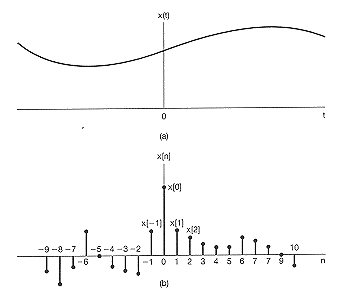
\includegraphics[scale=0.9]{pict/kontinudiskrit}
\caption{(a)Sinyal waktu-kontinu $x(t)$ dan (b)sinyal waktu-diskrit $x[n]$}\label{kontinudiskrit}
\end{figure}

\section{Transformasi Sinyal}
Konsep utama dalam analisa sinyal dan sistem adalah transformasi sinyal. Transformasi sinyal juga merupakan hal yang mendasar dan penting dalam pemrosesan sinyal terutam untuk melakukan manipulasi terhadap sinyal untuk menghilangkan sinyal yang tidak diinginkan ataupun menambahkan sesuatu pada sinyal sehingga menghasilkan sinyal yang sesuai dengan yang diinginkan. 
\subsection{Contoh-contoh transformasi variabel bebas}
Ada dua macam transformasi variabel bebas yang mendasar dan penting yaitu: pergeseran waktu (\textit{time shifting}) dan penskalaan waktu (\textit{time scaling}).
\begin{enumerate}
\item \textbf{pergeseran waktu}:\\
ambil sinyal waktu-kontinu $x(t)$, sinyal ini dapat digeser dengan pengurangan oleh faktor $t_0$
\[
x'(t)=x(t-t_0).
\] 
Jika $t_0>0$, sinyal $x(t)$ akan digeser ke kanan, atau terlambat (terjadi penundaan waktu/\textit{time delay}). Sedangkan jika $t_0<0$, maka $x(t)$ akan digeser ke kiri, atau mendahului. 

\begin{figure}[!h]
\centering
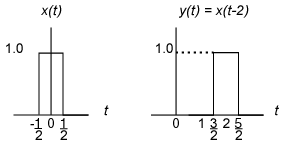
\includegraphics[scale=0.9]{pict/timeshift}
\caption{Gambaran operasi pergeseran waktu [2]}\label{timeshift}
\end{figure}

Untuk kasus sinyal diskrit $x[n]$, pergeseran waktu didefinisikan sebagai
\[
x'[n]=x[n-n_0],
\]
dengan $n_0$ yang juga harus merupakan bilangan bulat. Sama halnya dengan sinyal waktu-kontinu, jika $n_0$ positif maka sinyal tergeser ke kanan dan sebaliknya jika $n_0$ negatif maka sinyal tergeser ke kiri.

\item \textbf{penskalaan waktu}:\\
Sinyal yang didapatkan dengan menskalakan variabel bebas $t$ pada sinyal kontinu didefiniskan sebagai
\begin{equation}
x'(t)=x(at).
\end{equation} 
Untuk penskalaan waktu, jika $a>1$, maka sinyal akan terkompresi atau menyusut dari sinyal $x(t)$. Jika $0<a<1$, maka sinyal akan mengembang dari sinyal $x(t)$.

\begin{figure}[!h]
\centering
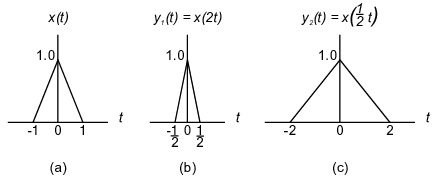
\includegraphics[scale=0.7]{pict/timescaling}
\caption{Operasi penskalaan waktu pada sinyal kontinyu $x(t)$ [2]}
\end{figure}

\begin{figure}[!h]
\centering
\begin{subfigure}[b]{0.4\textwidth}
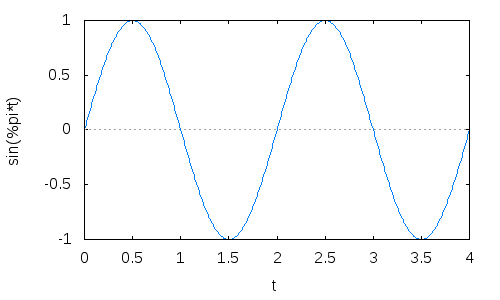
\includegraphics[width=\textwidth]{pict/timescaling1}
\caption{$x(t)=\sin \pi t$}
\end{subfigure}%
        ~ %add desired spacing between images, e. g. ~, \quad, \qquad etc.
          %(or a blank line to force the subfigure onto a new line)
\begin{subfigure}[b]{0.4\textwidth}
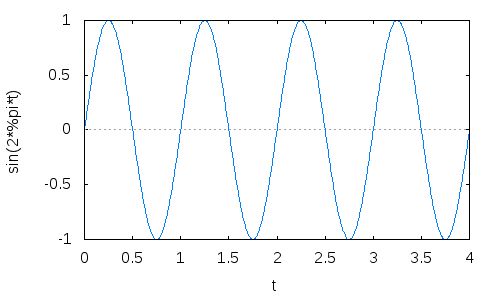
\includegraphics[width=\textwidth]{pict/timescaling2}
\caption{$x'_1(t)=\sin \pi 2t$}
\end{subfigure}
        ~ %add desired spacing between images, e. g. ~, \quad, \qquad etc.
          %(or a blank line to force the subfigure onto a new line)
\begin{subfigure}[b]{0.4\textwidth}
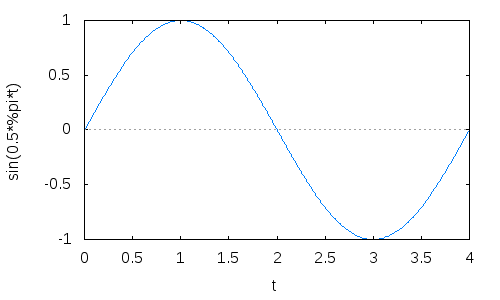
\includegraphics[width=\textwidth]{pict/timescaling3}
\caption{$x'_2(t)=\sin \pi \frac{t}{2}$}
\end{subfigure}
\caption{Efek penskalaan waktu pada sinyal sinusoidal}
\end{figure}

Untuk sinyal diskrit, penskalaan waktu didefinisikan sebagai
\begin{equation}
x'[n]=x[at]
\end{equation} 
\end{enumerate}
\subsection{Sinyal periodik}
Kelas sinyal penting yang akan sering kita jumpai dalam pemrosesan sinyal adalah sinyal periodik. Sinyal waktu-kontinu periodik $x(t)$ mempunyai sifat bahwa harga $T$-nya positif bagi
\begin{equation}
x(t) = x(t+T)
\end{equation}
untuk semua harga $t$.Sinyal periodik mempunyai sifat penting yaitu tidak berubah dengan pergeseran waktu $T$. Dalam persamaan (2.3) dikatakan bahwa $x(t)$ periodik dengan periode $T$. Jika $x(t)$ periodik dengan periode $T$, maka juga bisa dikatakan bahwa $x(t)=x(t+mT)$ untuk semua $t$ dan setiap bilangan bulat $m$. Dengan kata lain$x(t)$ juga periodik dengan periode $2T, 3T, 4T, ...$ Periode dasar $T_0$ pada $x(t)$ merupakan harga poditif terkecil $T$.

\begin{figure}[!h]
\centering
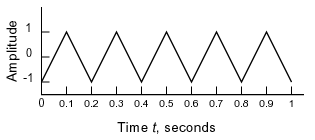
\includegraphics[scale=0.9]{pict/periodik}
\caption{Contoh sinyal periodik waktu-kontinu}
\end{figure}

Sinyal periodik pada waktu-diskrit didefinisikan sebagai
\begin{equation}
x[n]=x[n+N].
\end{equation}
Sinyal waktu diskrit $x[n]$ adalah periodik dengan periode $N$, dimana $N$ adalah bilangan bulat positif. 

\subsection{Sinyal genap dan sinyal ganjil}
Sinyal $x(n)$ atau $x[n]$ dikatakan sebagai sinyal genap jika identik terhadap waktu balikannya identik. Seperti bayangan pada cermin. Untuk sinyal waktu-kontinu didefinisikan sebagai
\begin{equation}
x(-t) = x(t),
\end{equation}
sedangkan untuk waktu-diskrit didefinisikan sebagai
\begin{equation}
x[-n]=x[n].
\end{equation}
Sinyal dikatakn sebagai sinyal ganjil jika
\begin{align}
x(-t) &= -x(t)\\
x[-n] &= -x[n].
\end{align}  
Sinyal ganjil harus 0 jika $x=0$ atau $n=0$.
\begin{figure}
\centering
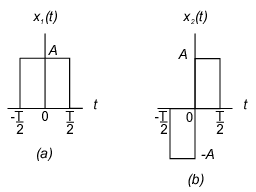
\includegraphics[scale=0.9]{pict/genapganjil}
\caption{Contoh sinyal genap (a) dan ganjil (b).}
\end{figure} 

\section{Sinyal Eksponensial dan Sinyal Sinusoidal Waktu-kontinu}
Sinyal eksponensial waktu-kontinu didefinisikan dalam bentuk umum
\begin{equation}
x(t)=Ce^{at}.
\end{equation}
Ada beberapa karakteristik berbeda yang dapat ditampilkan oleh sinyal eksponensial bergantung pada parameter $C$ dan $a$ yang dilimikinya, Karakteristik-karakteristik ini ditampilkan pada tabel 2.1 berikut

\begin{table}
\centering
\caption{Beberapa karakteristik sinyal eksponensial kompleks}
\begin{tabular}{|c|c|c|}
\hline
\textbf{Karakteristik} & $C$ & $a$\\
\hline
\hline
Sinyal eksponensial real & real & real\\
\hline
Sinyal eksponensial kompleks periodik & real & imajiner\\
\hline
Sinyal eksponensial kompleks umum & kompleks & kompleks\\
\hline
\end{tabular}
\end{table}
\subsection{Sinyal eksponensial real}
Sinyal eksponensial real mempunyai komponen $C$ dan $a$ berupa bilangan real. Bergantung pada apakah nilai $a$ positif atau negatif, sinyal eksponensial real terbagi menjadi sinyal eksponensial meningkat dan sinyal eksponensial meluruh.
\[
a>0\;\;\rightarrow \text{sinyal eksponensial meningkat}
\]
\[
a<0\;\;\rightarrow \text{sinyal eksponensial meluruh}
\]
\begin{figure}[!h]
\centering
\begin{subfigure}[b]{0.4\textwidth}
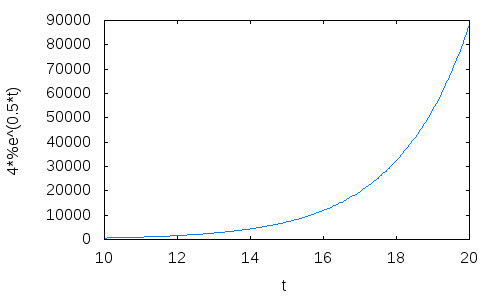
\includegraphics[width=\textwidth]{pict/exponensial1}
\caption{$x_1(t)=4e^{0,5t}$}
\end{subfigure}%
\begin{subfigure}[b]{0.4\textwidth}
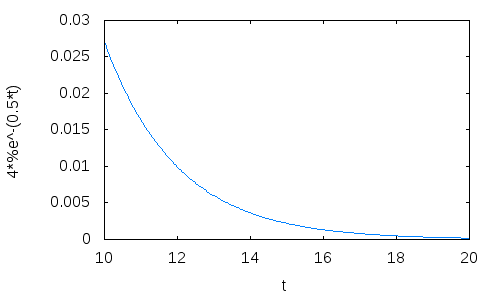
\includegraphics[width=\textwidth]{pict/exponensial2}
\caption{$x_2(t)=4e^{0,5t}$}
\end{subfigure}
\caption{Sinyal eksponensial meningkat (a) dan sinyal eksponensial meluruh (b)}
\end{figure}

\subsection{Sinyal eksponensial kompleks periodik}
Sinyal eksponensial kompleks periodik memiliki komponen $a$ yang imajiner. 
\begin{equation}
x(t)=e^{j\omega_0 t}
\end{equation}
Sinyal jenis ini bersifat periodik, jika kita tengok kembali persamaan (2.3) maka didapat bahwa
\[
e^{j\omega_0 t}=e^{j\omega_0 (t+T)}
\]
atau
\[
e^{j\omega_0(t+T)}=e^{j\omega_0 t} e^{j\omega_0 T}.
\]
Dari sini kita lihat bahwa suatu sinyal periodik jika 
\[
e^{j\omega_0 T} = 1.
\]
Sinyal eksponensial periodik memiliki periode dasar $T_0$,
\begin{equation}
T_0=\frac{2\pi}{|\omega_0|}.
\end{equation}
Sinyal $e^{j\omega_0 t}$ dan $e^{-j\omega_0 t}$ mempunyai periode dasar yang sama.

\subsection{Sinyal sinusoidal}
Secara umum sinyal sinusoidal didefinisikan sebagai
\begin{equation}
x(t) = A \cos (\omega_0 t + \phi),
\end{equation}
Dimana $A$ adalah amplituda sinyal, $\omega_0$ adalah frekuensi sudut dengan satuan radian per sekon, dan $\phi$ adalah fase dengan satuan radian. $\omega_0$ dapat ditulis sebagai
\[
\omega_0=2 \pi f_0,
\]
dimana $f_0$ adalah frekuensi dasar yang memiliki satuan putaran per sekon. Sinyal sinusoidal adalah sinyal periodik dengan periode dasar $T_0$. Sinyal sinusoidal memiliki hubungan dengan sinyal eksponensial periodik melalui hubungan Euler
\begin{equation}
e^{j\omega_0 t}=\cos \omega_0 t + j \sin \omega_0 t.
\end{equation}
Kita bisa mengekspresikan sinyal sinusoidal ke dalam komponen real dan imajiner eksponensial kompleksnya.
\begin{align}
A\cos (\omega_0 t+\phi)&=A \Re\lbrace e^{(j\omega_0t+\phi)}\rbrace\\
A\sin (\omega_0 t +\phi)&= A\Im\lbrace e^{(j\omega_0 t+\phi)}\rbrace. 
\end{align}
Selain itu, sinyal sinusoidal juga dapat dituliskan ke dalam sinyal eksponensial periodik melalui
\begin{equation}
A\cos (\omega_0 t+\phi)=\frac{A}{2}e^{j\phi}e^{j\omega_0 t} + \frac{A}{2} e^{-j \phi} e^{-j\omega_0 t}. 
\end{equation} 

\begin{figure}
\centering
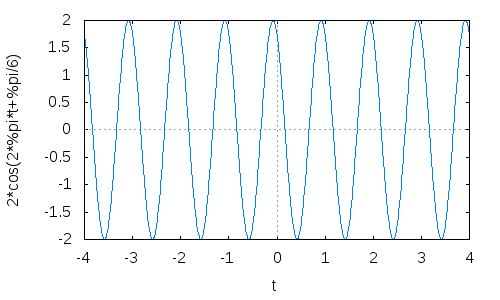
\includegraphics[scale=0.4]{pict/sinusoidal}
\caption{Contoh sinyal sinusoidal $x(t)=2\cos (2\pi t+\frac{\pi}{6})$}
\end{figure}

\subsection{Sinyal eksponensial kompleks umum}
Sinyal eksponensial kompleks umum memilik komponen $C$ dan $a$ berupa bilangan kompleks. Dalam hal ini $C$ diekspresikan ke dalam bentuk polar ($re^{j \phi}$), sedangkan $a$ ke dalam bentuk rektangular ($x+jy$). 
\begin{align*}
C&=|C|e^{j\phi}\\
a&=r+j\omega_0.
\end{align*}
Maka sinyal eksponensial kompleks umum dituliskan sebagai
\begin{equation}
Ce^{at}=|C|e^{j\phi}e^{(r+j\omega_0)}=|C|e^{rt}e^{j(\omega_0 t+\phi)}.
\end{equation}
Dengan menggunakan hubungan Euler, kita dapat memperluasnya menjadi
\begin{equation}
Ce^{at}=|C|e^{rt} \cos(\omega_0 t+\phi)+j|C|e^{rt}\sin(\omega_0 t+\phi).
\end{equation}
Untuk nilai $r$, jika
\begin{align*}
r=0\;\;&\rightarrow \text{bagian real dan imajiner eksponensial kompleks adalah sinusoidal}\\
r>0\;\;&\rightarrow \text{sinyal sinusoidal meningkat}\\
r<0\;\;&\rightarrow \text{sinyal sinusoidal meluruh atau teredam}
\end{align*}

\begin{figure}[!h]
\centering
\begin{subfigure}[b]{0.5\textwidth}
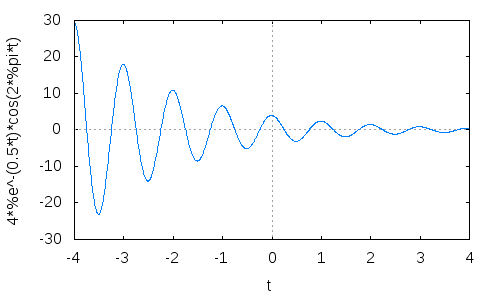
\includegraphics[width=\textwidth]{pict/sinusturun}
\caption{$x_1(t)=4e^{-0,5t}\cos(2\pi t)$}
\end{subfigure}%
\begin{subfigure}[b]{0.5\textwidth}
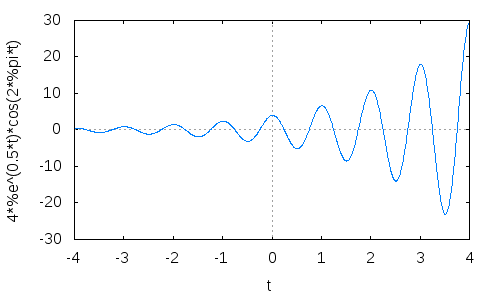
\includegraphics[width=\textwidth]{pict/sinusnaik}
\caption{$x_2(t)=4e^{0,5t}\cos(2\pi t)$}
\end{subfigure}
\caption{Sinyal sinusoidal meningkat (a) dan sinyal sinusoidal meluruh atau teredam (b).}
\end{figure}

\section{Sinyal Eksponensial Kompleks dan Sinyal Sinusoidal Kompleks Waktu-Diskrit}

%===============================================================
\chapter{Analisa Sistem Tak Ubah Waktu}

\section{Pengantar}
Sinyal dan sistem merupakan sebuah kesatuan yang saling berhubungan satu sama lain. Sinyal merupakan pola-pola bervariasi yang berubah terhadap satu atau lebih variabel bebas, yang berisi informasi tentang perilaku atau sifat dari suatu fenomena tertentu. Sistem akan menerima sinyal untuk kemudian mengelola, mengolahnya sehingga menhasilkan keluaran atau tanggapan berupa sinyal lain ataupun perilaku atau sifat tertentu sesuai keinginan. Penerapan sinyal dan sistem ada dalam banyak bidang yang bervariasi mulai dari teknologi komunikasi, elektronika, komputer, pembangkit energi, pengolahan suara untuk musik, transportasi, sampai kendali otomatis pada proses-proses di industri. Masih banyak lagi penerapan sinyal dan sistem dalam kehidupan sehari-hari yang kita sadari atau tidak telah kita gunakan secara rutin dalam kehidupan kita. Penerapan-penerapan tersebut kesemuanya memiliki pola dan ciri mendasar seperti yang telah dijabarkan pada awal paragraf. Contoh sederhananya adalah mobil. Mobil bergerak dan melaju dengan kecepatan tertentu akibat adanya injakan dari pedal gas, dalam hal ini injakan pada pedal gas merupakan sinyal masukan bagi sistem mobil dan sistem mobil melalui proses mekanis dan termodinamik pada mesinnya akan menhasilkan tanggapan berupa laju mobil yang sesuai dengan seberapa dalam injakan pedal gas. Contoh lain terdapat pada rangkaian listrik, dimana sinyal masukan berupa arus dan tegangan listrik yang berubah terhadap waktu pada sistem rangkaian listrik yang dapat berupa komponen-komponen elektronik dan elektrik seperi resistor, kapasitor dan lain-lain akan menghasilkan tanggapan berupa arus dan tegangan yang berbeda sesuai dengan yang diinginkan. 

\begin{figure}[!h]
\centering
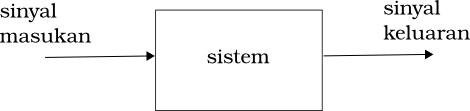
\includegraphics[scale=0.7]{pict/sinyalsistem}
\caption{Representasi konsep sinyal dan sistem dalam diagram blok}\label{sinyalsistem}
\end{figure}

Konsep sinyal dan sistem muncul dalam dalam berbagai aplikasi yang berbeda bergantung pada bagaimana pengunaan konsep tersebut. Konsep sinyal dan sistem dapat digunakan untuk mengkaraterisasi sebuah sistem. Mengkarakterisasi berarti membaca karakter atau sifat dari sebuah sistem tertentu dengan cara memberikan sinyal masukan yang bervariasi dan membaca bagaimana sistem menanggapai masukan yang bervariasi tersebut. Hal ini seperti apabila kita mempunyai sebuah kotak hitam yang kita tidak tahu sepeti apa sifat dan bagaimana kotak hitam tersebut bekerja. Dengan memberikan masukan bervariasi terhadap kotak hitam tersebut maka akan dapat diperoleh keluaran barupa tanggapan yang berbeda dengan masukan, sehingga dengan ini kita dapat mengetahui apa dan bagaimana kotak hitam misterius ini berperilaku atau bekerja. Konsep sinyal dan sistem juga dapat digunakan untuk melakukan pemrosesan terhadap sinyal tertentu agar diperoleh keluaran sinyal sesuai yang diharapkan atau untuk menghilangkan sinyal yang tidak diinginkan. Contohnya adalah dalam sistem \textit{noise canceling} (NC) atau pembatal bising. Dalam sistem NC yang biasa digunakan pada speaker, bising atau suara mengganggu yang tidak diinginkan dari dapat diredam sedemikian hinga sehingga suara atau bunyi yang keluar dari \textit{speaker} adalah ahanya suara yang diharapkan. Sistem NC akan membangkitkan suara dengan frekuensi tertentu yang sama dengan suara bising tertentu tetapai dengan fase yang berbeda sehingga melalui proses interferensi suara bising dapat diredam. 


%==============================================================
\chapter{Deret Fourier Fungsi Periodik}

\section{Pengantar}
Fungsi periodik banyak ditemui dalam berbagai masalah teknik. Fungsi tersebut biasanya lebih rumit daripada fungsi sinus dan kosinus. Deret Fourier merupakan upaya untuk menyatakan sembarang fungsi periodik kedalam fungsi sinus dan kosinus.

Suatu fungsi dinyatakan periodik jika fungsi tersebut terdefinisikan untuk semua $x$ real dan jika terdapat bilangan positif T sedemikian hingga

\begin{equation}
\label{sec:periodik}
f(x+T)=f(x),  
\end{equation}
untuk semua $x$.

Bilangan T disebut periode dari fungsi $f(x)$. Menurut persamaan~\ref{sec:periodik} jika $n$ bilangan bulat  sembarang, maka berlaku

Konsep sinyal dan sistem muncul dalam dalam berbagai aplikasi yang berbeda bergantung pada bagaimana pengunaan konsep tersebut. Konsep sinyal dan sistem dapat digunakan untuk mengkaraterisasi sebuah sistem. Mengkarakterisasi berarti membaca karakter atau sifat dari sebuah sistem tertentu dengan cara memberikan sinyal masukan yang bervariasi dan membaca bagaimana sistem menanggapai masukan yang bervariasi tersebut. Hal ini seperti apabila kita mempunyai sebuah kotak hitam yang kita tidak tahu sepeti apa sifat dan bagaimana kotak hitam tersebut bekerja. Dengan memberikan masukan bervariasi terhadap kotak hitam tersebut maka akan dapat diperoleh keluaran barupa tanggapan yang berbeda dengan masukan, sehingga dengan ini kita dapat mengetahui apa dan bagaimana kotak hitam misterius ini berperilaku atau bekerja. Konsep sinyal dan sistem juga dapat digunakan untuk melakukan pemrosesan terhadap sinyal tertentu agar diperoleh keluaran sinyal sesuai yang diharapkan atau untuk menghilangkan sinyal yang tidak diinginkan. Contohnya adalah dalam sistem \textit{noise canceling} (NC) atau pembatal bising. Dalam sistem NC yang biasa digunakan pada speaker, bising atau suara mengganggu yang tidak diinginkan dari dapat diredam sedemikian hinga sehingga suara atau bunyi yang keluar dari \textit{speaker} adalah ahanya suara yang diharapkan. Sistem NC akan membangkitkan suara dengan frekuensi tertentu yang sama dengan suara bising tertentu tetapai dengan fase yang berbeda sehingga melalui proses interferensi suara bising dapat diredam. 


%===============================================================
\include{bab4_transformfourier}
%==============================================================
\include{bab5_aplikasi}
%===============================================================
%===============================================================
\chapter*{Apendiks A :\\ Kalkulus Diferensial dan Kalkulus Integral}
\section{Kalkulus Diferensial}
Fenomena fisis seringkali berurusan dengan sesuatu yang berubah terhadap waktu atau dengan kata lain berubah secara kontinu. Matematika kalkulus digunakan untuk berurusan dengan hal-hal yang berkenaan dengan perubahan kontinu. Kalkulus berhubungan dengan limit. Untuk memahami ide tentang limit, bayangakan kita memiliki urutan bilangan $l_1, l_2, l_3,...$ yang nilainya semakin dekat dan semakin dekat dengan sebuah nilai $L$. Sebagai contoh: 0.9, 0.99, 0.999, 0.9999,..... Dapat dikatakan bahwa limit dari urutan ini adalah sama dengan 1. Tidak ada satu pun dari angka-angka tersebut yang sama dengan 1, akan tetapi semakin lama semakin mendekati nilai 1. Jika ide ini digunakan pada fungsi yang berubah sejalan dengan waktu $f(t)$, maka $L$ adalah limit dari fungsi ketika $t$ mendekati nilai tertentu, misalnya $a$.
%--------------------------------------------------------------
\begin{equation}
\lim_{t\rightarrow a}f(t)=L 
\end{equation}
%--------------------------------------------------------------
Kalkulus diferensial berhubungan dengan laju perubahan fungsi $\Delta f$ terhadap perubahan waktu $\Delta t$. Laju perubahan didefinisikan sebagai rasio dari perubahan fungsi $\Delta f$ terhadap perubahan waktu $\Delta t$. Sepanjang interval $\Delta t$, fungsi berubah dari $f(t)$ menjadi $f(t+\Delta t)$, sehingga
\begin{equation}
\Delta f = f(t+\Delta t) - f(t)
\end{equation}
%--------------------------------------------------------------
\begin{figure}[!h]
\centering
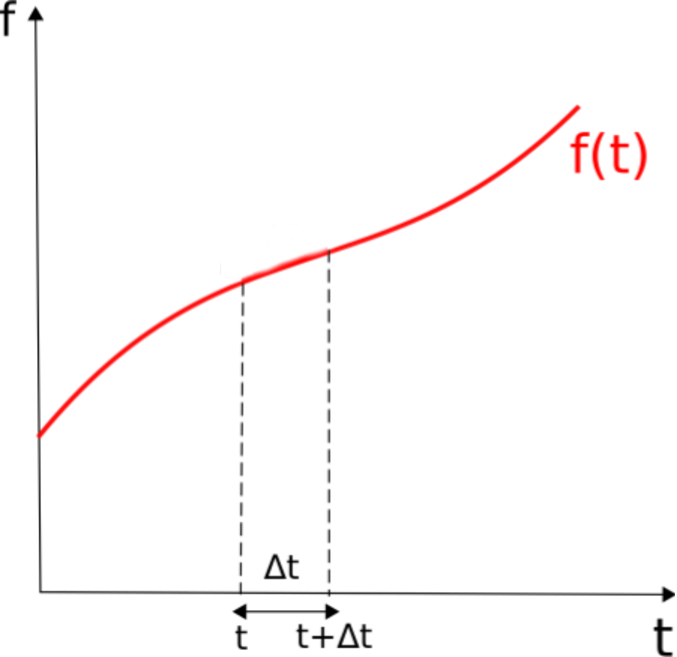
\includegraphics[scale=0.6]{pict/differentialgraph.pdf}
\caption{Grafik fungsi yang berubah terhadap waktu, $\Delta f$ menunjukkan perubahan dalam fungsi sedangkan $\Delta t$ menunjukkan perubahan dalam waktu}\label{differential}
\end{figure}
%--------------------------------------------------------------
Untuk mendefinisikan laju perubahan pada satu waktu $t$ secara lebih akurat, kita harus menyusutkan $\Delta t$ pada Gambar 1.1 sampai nol. Tentu saja jika kita menyusutkan $\Delta t$ hingga nol maka $\Delta f$ juga akan menjadi nol. Akan tetapi, jika kita membagi $\Delta f$ dengan $\Delta t$ maka rasio/pembagian tersebut akancenderung menuju sebuah limit. Limit tersebut adalah turunan/derivatif dari fungsi $f(t)$ terhadap waktu $t$.
\begin{equation}
\label{sec:turunan}
\frac{df}{dt}=\lim_{\Delta t \rightarrow 0} \frac{\Delta f}{\Delta t}=\lim_{\Delta t \rightarrow 0} \frac{f(t + \Delta t)-f(t)}{\Delta t}.
\end{equation}
Sebagai contoh kita hitung turunan dari fungsi $f(t)=t^2$. Kita gunakan persamaan~\ref{sec:turunan} untuk menghitungnya, dimulai dari :
\[
f(t+\Delta t)=(t+\Delta t)^2=t^2+2t\Delta t + \Delta t^2
\]
kemudian kurangkan dengan $f(t)$
\begin{align*}
f(t+\Delta t)-f(t)&=t^2+2t\Delta t + \Delta t^2 - t^2\\
&=2t\Delta t + \Delta t^2.
\end{align*}
Dengan membaginya dengan $\Delta t$, kita dapatkan:
\begin{align*}
\frac{f(t + \Delta t)-f(t)}{\Delta t}&=\frac{2t\Delta t + \Delta t^2}{\Delta t}\\
&=2t+\Delta t.
\end{align*}
Pembagian ini akan menghasilkan limit jika $\Delta t \rightarrow 0$:
\begin{align*}
\lim_{\Delta t\rightarrow 0}\frac{f(t+\Delta t)-f(t)}{\Delta t}&=\lim_{\Delta t \rightarrow 0} 2t + \Delta t\\
&= 2t.
\end{align*} 
Jadi, turunan dari $t^2$ adalah
\[
\frac{d(t^2)}{dt}=2t
\]
Selanjutnya untuk fungsi dengan perpangkatan secara umum $f(t)=t^n$, turunannya dapat dihitung dengan memanfaatkan teorema binomial
\[
(a+b)^n=a^n+na^{n-1}b+\frac{n(n-1)}{2}a_{n-2}b^2+\frac{n(n-1)(n-2)}{3}a^{n-3}b^3+...+b^n.
\] 
Dengan menggunakan teorema binomial ini kita dapat menghitung $f(t+\Delta t)$,
\begin{align*}
f(t+\Delta t)&=(t+\Delta t)^n\\
&=t^n+nt^{n-1}\Delta t+...
\end{align*}
pengurangan dengan $f(t)$ menghasilkan
\begin{align*}
\Delta f&= f(t+\Delta t)-f(t)\\
&= t^n+nt^{n-1}\Delta t+\frac{n(n-1)}{2}t{n-2}\Delta t^2+...-t^n\\
&=nt^{n-1}\Delta t+\frac{n(n-1)}{2}t^{n-2}\Delta t^2+...
\end{align*}
Kemudian membaginya dengan $\Delta t$,
\[
\frac{\Delta f}{\Delta t}=nt^{n-1}+\frac{n(n-1)}{2}t^{n-2}\Delta t+...
\]
Dengan $\Delta t \rightarrow 0$ maka semua bagian yang mengandung $\Delta t$ akan menyusut menjadi nol dan menghasilkan sebuah limit
\begin{equation}
\frac{d(t^n)}{dt}=nt^{n-1},
\end{equation}
yang merupakan rumusan umum praktis untuk menyelesaikan turunan fungsi perpangkatan. $n$ di sini tidak terbatas pada bilangan bulat, tetapi juga untuk bilangan real apapun atau bahkan bilangan kompleks.

Beberapa aturan dalam turunan:
\begin{enumerate}
\item Turunan dari sebuah konstanta (konstanta adalah angka apapun, baik bilangan bulat maupun bilangan real) adalah sama dengan nol. Hal ini benar menurut pengertian turunan, yaitu bahwa turunan adalah laju perubahan, dan sebuah konstanta tidak akan berubah:
\[
\frac{dc}{dt}=0
\]
\item Turunan dari sebuah konstanta dikalikan dengan sebuah fungsi adalah konstanta tersebut dikalukan turunan dari fungsi:
\[
\frac{(cf)}{dt}=c\frac{df}{dt}
\]
\item Penjumlahan dari dua fungsi $f(t)$ dan $g(t)$ adalah juga berupa fungsi dan turunannya diberikan oleh:
\[
\frac{d(f+g)}{dt}=\frac{d(f)}{dt}+\frac{d(g)}{dt}.
\]
Aturan ini disebut dengan \textit{aturan penambahan} atau \textit{sum rule}.
\item Hasil kali dari dua fungsi adalah juga berupa fungsi dan turunannya adalah:
\[
\frac{d(fg)}{dt}=f(t)\frac{d(g)}{dt}+g(t)\frac{d(f)}{dt}.
\]
Aturan ini disebut \textit{aturan hasil kali}.
\item Jika kita memiliki dua fungsi, dimana $g(t)$ adalah sebuah fungsi dari $t$ dan $f(g)$ adalah fungsi dari $g$, yang membuat $f$ secara tidak langsung merupakan fungsi dari $t$. Maka untuk menurunkan fungsi semacam ini pertama kita harus turunkan terlebih dahulu fungsi $g(t)$ untuk kemudian barulah menurunkan $f(g)$:
\[
\frac{df}{dt}=\frac{df}{dg}\frac{dg}{dt}
\]
Aturan ini disebut dengan \textit{aturan rantai}. Hal yang penting dalam aturan rantai adalah bahwa kita harus menemukan fungsi perantara $g(t)$ untuk dapat menyederhanakan $f(t)$ dan membuatnya menjadi $f(g)$. Sebagai contoh, kita ambil fungsi $f(t)=\ln t^3$. Dalam fungsi ini $t^3$ bisa menjadi sebuah masalah. Kita ambil $t^3$ di dalam logaritma sebagai fungsi perantara, $g=t^3$. Sehingga sekarang kita memiliki $f(g)=\ln g$. Turunan kedua fungsi adalah:
\begin{align*}
\frac{df}{dt}&=\frac{1}{g}, dan\\
\frac{dg}{dt}&=3t^2.
\end{align*}
Dengan menggunakan aturan rantai, kita dapatkan:
\begin{align*}
\frac{df}{dt}&=\frac{df}{dg}\frac{dg}{dt}\\
&=\frac{3t^2}{g}.
\end{align*}
Substitusi $g=t^3$ menghasilkan turunan dari fungsi $f(t)$ terhadap waktu $t$
\[
\frac{df}{dt}=\frac{3t^2}{t^3}=\frac{3}{t}
\]   
\end{enumerate}
\section{Kalkulus Integral}
Jika kalkulus diferensial berhubungan dengan laju perubahan. kalkulus integral berhubungan dengan jumlahan dari banyak bagian-bagian kecil. Masalah utama dalam kalkulus integral adalah menghitung luasan dibawah kurva yang didefinisikan oleh sebuah fungsi $f(t)$. Misalkan kita ingin menghitung luasan dibawah kurva fungsi $f(t)$ dengan batasan dari a sampai b. Maka sebagai pendekatan kita dapat pecah-pecah luasan tersebut ke dalam bagian-bagian yang lebih kecil berbentuk persegi panjang dengan masing-masing memiliki ukuran yang sama, seperti terlihat pada gambar 1.2.
%-------------------------------------------------------------- 
\begin{figure}[!h]
\centering
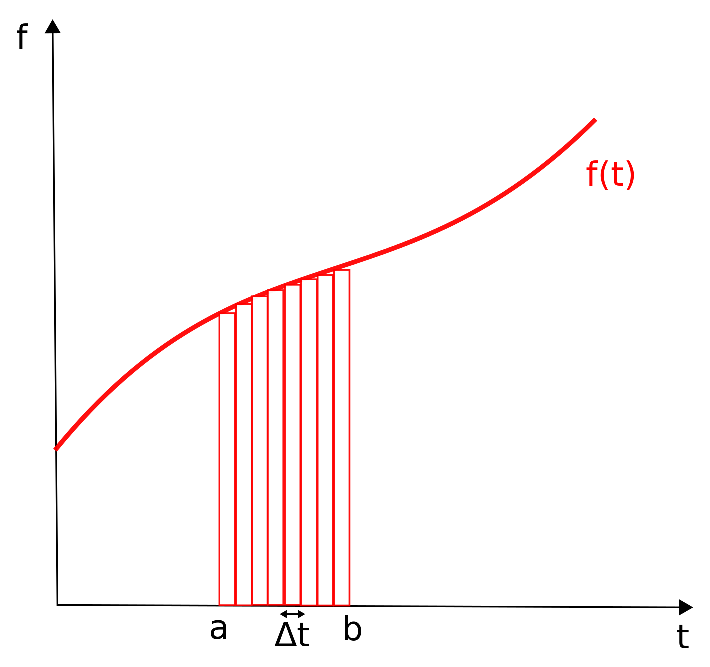
\includegraphics[scale=0.6]{pict/integralgraph.eps}
\caption{Grafik fungsi yang berubah terhadap waktu, Luasan di bawah kurva fungsi $f(t)$ dibagi-bagi kedalam banyak sub-luasan lebih kecil berbentuk persegi panjang}\label{integral}
\end{figure}
%--------------------------------------------------------------
Lebar dari persegi panjang ini adalah $\Delta t$ dan tingginya merupakan nilai lokal dari fungsi $f(t)$. Luasan dari sebuah persegi panjang tersebut adalah:
\[
\delta A=f(t)\Delta t
\]
Sekarang kita jumlahkan tiap-tiap persegi panjang ini sehingga mendekati luasan di bawah kurva dari a ke b.
\[
A=\sum^N_i f(t_i)\Delta t,
\]
$N$ di sini adalah banyaknya bagian-bagian persegi panjang. Untuk memperoleh hasil yang tepat dari luasan di bawah kurva ini, maka kita susutkan $\Delta t$ hingga menjadi nol dan jumlah dari persegi panjang menjadi tak berhingga. Integral tertentu antara $t=a$ dan $t=b$ dituliskan sebagai
\[
A=\int^b_a f(t) dt =\lim_{\Delta t \rightarrow 0} \sum_i f(t_i) \Delta t.
\]
Tanda integral $\int$, disebut \textit{summa}, menggantikan tanda penjumlahan sigma, dan $\Delta t$ digantikan oleh $dt$. Fungsi $f(t)$ disebut sebagai \textit{integrand}.

Jika kita ganti batasan $b$ dengan nilai variabel $T$ sehingga integrasi menjadi tak tentu. 
\[
\int^T_a f(t) dt
\]
Integral ini direpresentasikan dalam fungsi $F(T)$. Fungsi $F(T)$ mendefinisikan integral tak tentu dari fungsi $f(t)$, biasa ditulis dengan
\begin{equation}
F(T)=\int f(t) dt.
\end{equation}

Hubungan antara integral dan turunan bersifat resiprokal, yang berarti bahwa turunan dari integral adalah \textit{integrand} itu sendiri
\[
\frac{dF}{dt}=f(t).
\]
Hal ini dapat dibuktikan dengan menambahkan perubahan bagian kecil persegi panjang pada $T$ dari $T$ sampai $T+\Delta t$, sehinggga kita memiliki integral baru
\[
F(T+\Delta t)=\int^{T+\Delta t}_a f(t)dt.
\]  
Dengan penambahan sebuah persegi panjang Perbedaan $F(T+\Delta t)-F(T)$ tak lain hanyalah luasan dari persegi panjang tambahan itu sendiri
\[
F(T+\Delta t)-F(T)=f(T)\Delta t
\]
Pembagian dengan $\Delta t$ menghasilkan
\[
\frac{F(T+\Delta t)-F(T)}{\Delta t}=f(T).
\]
Jika kita ambil limit dimana $\Delta t \rightarrow 0$, maka
\[
\frac{dF}{dT}=\lim_{\Delta t \rightarrow 0} \frac{F(T+\Delta t)-F(T)}{\Delta t}=f(T).
\]  
Kita dapat menyederhanakan ini dengan mengabaikan perbedaan antara $t$ dan $T$,
\[
\frac{dF}{dt}=f(t).
\]

Untuk lebih memahaminya kita coba menemukan integral dari fungsi perpangkatan $f(t)=t^n$
\[
F(t)=\int f(t)dt=\int t^n dt.
\]
Dari hubungan antara $F$ dan $f$
\[
f(t)=\frac{dF(t)}{dt}
\]
atau
\[
t^n=\frac{dF(t)}{dt}.
\]
Hal yang harus kita lakukan adalah menemukan fungsi $F$ yang turunannya adalah $t^n$.\\
Dari sub-bab sebelumnya tentang kalkulus diferensial, kita menemukan bahwa untuk apapun nilai $m$,
\[
\frac{d(t^m)}{dt}=mt^{m-1}
\].
Jika kita substitusikan $m=n+1$, maka akan menjadi
\[
\frac{d(t^{n+1})}{dt}=(n+1)t^n
\]
atau, dengan membagi dengan $n+1$,
\[
\frac{d(\frac{t^{n+1}}{n+1})}{dt}=t^n.
\]
Sehingga kita menemukan bahwa $t^n$ adalah turunan dari $\frac{t^{n+1}}{n+1}$. Dapat dituliskan sebagai
\[
F(t)=\int t^n dt=\frac{t^{n+1}}{n+1}.
\]

Secara umum teorema dasar dari kalkulus dapat dituliskan sebagai
\begin{equation}
\int^b_af(t)dt=F(t)\vert^b_a=F(b)-F(a).
\end{equation}

Beberapa rumus integrasi antara lain:
\begin{itemize}
\item $\int cdt=ct$
\item $\int cf(t)dt=c\int f(t) dt$
\item $\int t dt=\frac{t^2}{2}+c$
\item $\int t^2dt=\frac{t^3}{3}+ c$
\item $\int t^ndt=\frac{t^{n+1}}{n+1}+c$
\item $\int \sin tdt=-\cos t+c$
\item $\int \cos tdt=\sin t+c$
\item $\int e^t dt=e^t$
\item $\int \frac{dt}{t}=\ln t+c$
\item $\int [f(t)\pm g(t)]dt=\int f(t) dt \pm \int g(t) dt$. 
\end{itemize}

\subsubsection{Integrasi parsial}
Integrasi parsial adalah salah satu \textit{tool} untuk menyelesaiakn perhitungan integral yang rumit. Integral parsial merupakan balikan dari \textit{aturan hasil kali} dari turunan. Kembali kita tinjau \textit{aturan hasil kali}
\[
\frac{d[f(x)g(x)]}{dx}=f(x)\frac{dg(x)}{dx}+g(x)\frac{df(x)}{dx}.
\]
Mengintegralkan kedua sisi dari presamaan dari $a$ sampai $b$ menghasilkan
\begin{align}
\int_a^b\frac{d[f(x)g(x)]}{dx}&=\int_a^bf(x)\frac{dg(x)}{dx}+\int_a^b g(x) \frac{f(x)}{dx}\\
f(x)g(x)\vert_a^b - \int_a^b f(x) \frac{dg(x)}{dx} &= \int_a^b g(x) \frac{df(x)}{dx}.
\end{align}
Jika $f(x)$ direpresentasikan dengan $u$ dan $g(x)$ dengan $v$, sehingga $df(x)/dx=du$ dan $dg(x)/dx=dv$, maka substitusi pada persamaan (1.8) menghasilkan
\begin{equation}
uv-\int udv = \int vdu,
\end{equation} 
yang merupakan rumusan praktis dari integrasi parsial. Sebagai contoh, kita hitung integral dari $x\cos x$ dari 0 sampai $\pi/2$
\[
\int_0^{\pi/2} x \cos x dx,
\]
dengan menggunakan persamaan (1.9) ambil $x$ sebagai $v$ dan $\cos x dx$ sebagai $du$
\begin{align*}
v&=x,  dv=dx\\
du&=\cos x dx,   u=\sin x.
\end{align*}  
Substitusi ke persamaan (1.9) menghasilkan
\begin{align*}
\int_0^{\pi /2} x \cos x dx&=x \sin x\vert_0^{\pi /2}-\int_0^{\pi /2} \sin x dx\\
&= \frac{\pi}{2} \sin \frac{\pi}{2}+\cos \frac{\pi}{2}\\
&=\frac{\pi}{2}.
\end{align*}

\end{document} 
